%; whizzy paragraph -pdf xpdf -latex ./whizzypdfptex.sh
%; whizzy-paragraph "^\\\\begin{frame}"
% latex beamer presentation.
% platex, latex-beamer でコンパイルすることを想定。 

%     Tokyo Debian Meeting resources
%     Copyright (C) 2009 Junichi Uekawa

%     This program is free software; you can redistribute it and/or modify
%     it under the terms of the GNU General Public License as published by
%     the Free Software Foundation; either version 2 of the License, or
%     (at your option) any later version.

%     This program is distributed in the hope that it will be useful,
%     but WITHOUT ANY WARRANTY; without even the implied warranty of
%     MERCHANTABILITY or FITNESS FOR A PARTICULAR PURPOSE.  See the
%     GNU General Public License for more details.

%     You should have received a copy of the GNU General Public License
%     along with this program; if not, write to the Free Software
%     Foundation, Inc., 51 Franklin St, Fifth Floor, Boston, MA  02110-1301 USA

\documentclass[cjk,dvipdfmx,12pt]{beamer}
\usetheme{Tokyo}
\usepackage{monthlypresentation}

%  preview (shell-command (concat "evince " (replace-regexp-in-string "tex$" "pdf"(buffer-file-name)) "&"))
%  presentation (shell-command (concat "xpdf -fullscreen " (replace-regexp-in-string "tex$" "pdf"(buffer-file-name)) "&"))
%  presentation (shell-command (concat "evince " (replace-regexp-in-string "tex$" "pdf"(buffer-file-name)) "&"))

%http://www.naney.org/diki/dk/hyperref.html
%日本語EUC系環境の時
\AtBeginDvi{\special{pdf:tounicode EUC-UCS2}}
%シフトJIS系環境の時
%\AtBeginDvi{\special{pdf:tounicode 90ms-RKSJ-UCS2}}

\title{東京エリア Debian 勉強会}
\subtitle{資料}
\author{上川 純一 dancer@debian.or.jp\\IRC nick: dancerj}
\date{2009年6月20日}
\logo{
\includegraphics[width=8cm]{image200607/openlogo-light.eps}}

\begin{document}

\frame{\titlepage{}}

\emtext{設営準備にご協力ください}

\begin{frame}{今日の参加の目標}
\begin{itemize}
 \item 荒木 靖宏: DDTSS の勉強をしにきました(1997年以来なので)
 \item 吉田@板橋: 小江戸LUGでDDTSSを紹介して好評だった、細かいところがよ
       くわからない。レビューばかりだったが翻訳は今回がはじめて。ご意見
       いただきたい。事前課題を出していないのは家のLennyがPDFを生成できなかっ
       たため。JOSMの翻訳をしてみた。
 \item かわもと: YLUGには結構でていて、初めてのひとはいないぜ。横浜在住
       なので荻窪が遠い。わかんないところもあるので、定期的にやってみた
       いので参加したい。
 \item やまね: くること! DDTSS のインタフェースは悪いよねぇ・・・。
       目が増えるといいんじゃね?
\end{itemize}
\end{frame}

\begin{frame}{今日の参加の目標}
\begin{itemize}
 \item キタハラ: DDTSS使ったのだが、とりあえず宿題までやったのだけど、よ
       くわからない。
 \item 日比野: pending review が大量にあるので、短いやつを適当にレビュー
       しまくった。作業者同士の意思疎通が必要かなとおもって今日きました。
 \item masaka: DDTSSの話をきいてちょっとやってみてわからなかったので教わ
       りにきました。
 \item 前田: 会場の手配と二次会の手配が完了しました。
 \item よしの: 先月のおわりころから DDTSS について日比野さんにだまされて
       レビューを100くらいやってみました。y\_yは実はぼくでした。
\end{itemize}
\end{frame}

\begin{frame}{今日の参加の目標}
\begin{itemize}
 \item あけど: DDTSS 数をこなしてみたぜ!自分の性に合うので続けたい。今日
       はTIPSを紹介したい。翻訳のポリシーとか決まってないところもあるの
       で議論したい。
 \item 山本浩之: 翻訳はむいていないことがわかったので、レビューを頑張ってい
       る.
 \item Norbert Preining:
 \item でんさん:
\end{itemize}
\end{frame}

\begin{frame}{会場費についての悲しいおしらせ}

500円予定とアナウンスしましたが、本日の会場は高いので割り勘すると1000円です。

\end{frame}

\section{}
\begin{frame}
 \frametitle{Agenda}
\begin{minipage}[t]{0.45\hsize}
  \begin{itemize}
  \item 注意事項
	\begin{itemize}
	 \item 持ち込み禁止
	 \item そこで購入した飲み物 OK
	 \item 食事禁止
	 \item Wireless AP は ``MacBook''
	\end{itemize}
  \item 最近あったDebian関連のイベント報告
	\begin{itemize}
	 \item 前回の勉強会
	\end{itemize}
 \end{itemize}
\end{minipage} 
\begin{minipage}[t]{0.45\hsize}
 \begin{itemize}
  \item DDTSS ワークショップ
  \item bsdstats を Debianize してみた
  \item Debian kFreeBSD
 \end{itemize}
\end{minipage}
\end{frame}

\section{最近}

\begin{frame}
 \frametitle{2009年5月}
\begin{minipage}[t]{0.45\hsize}
  \begin{itemize}
  \item 注意事項
	\begin{itemize}
	 \item ごみは持ち帰りましょう。
	 \item となりで三味線をひいているので、おおきな声はだすな。
	\end{itemize}
  \item 最近あったDebian関連のイベント報告
	\begin{itemize}
	 \item 前回の勉強会
	\end{itemize}
 \end{itemize}
\end{minipage} 
\begin{minipage}[t]{0.45\hsize}
 \begin{itemize}
  \item Erlang
  \item MC-MPIパッケージの道
  \item Andoidネタ
  \item DDTSS翻訳プロセスワークショップ
 \end{itemize}
\end{minipage}
\end{frame}

\begin{frame}{Hack Cafe}

毎週水曜日、週に一回東京のどっかのカフェでハック。

\end{frame}

\section{DWN quiz}
\begin{frame}{Debian 常識クイズ}

Debian の常識、もちろん知ってますよね?
知らないなんて恥ずかしくて、知らないとは言えないあんなことやこんなこと、
みんなで確認してみましょう。

今回の出題範囲は\url{debian-devel-announce@lists.debian.org} に投稿された
内容とDebian Project Newsからです。

\end{frame}

\subsection{問題}
%; whizzy-master ../debianmeetingresume200906.tex
% $B0J>e$N@_Dj$r$7$F$$$k$?$a!"$3$N%U%!%$%k$G(B M-x whizzytex $B$9$k$H!"(Bwhizzytex$B$,MxMQ$G$-$^$9!#(B
%
% $B$A$J$_$K!"%/%$%:$OJL%V%i%s%A$G:n@.$7!"$N$A$K%^!<%8$7$^$9!#5U$K%^!<%8$7(B
% $B$J$$$h$&$K$7$^$7$g$&!#(B
% (shell-command "git checkout quiz-prepare")

\santaku
{$B%h!<%m%C%Q$K?7@_$5$l$?%"%C%W%m!<%I%-%e!<$NL>A0$O(B?}
{ftp.eu.upload.debian.org}
{ftp.uk.upload.debian.org}
{ftp.jp.debian.org}
{A}
{}

\santaku
{$B?7$7$$%"%C%W%m!<%I%-%e!<$G?7$7$/%5%]!<%H$9$k$3$H$K$J$kDL?.%W%m%H%3%k$O(B?}
{ipv6}
{sstp}
{RFC2324} % coffee protocol
{A}
{}

\santaku
{GPG $B%-!<:F:n@.:W$j$O$J$<H/@8$7$?$+(B?}
{$B$=$m$=$m(Bsha-1$B$,@H<e$K$J$C$?$H;W$o$l$k$+$i(B}
{$BOG@1$,D>Ns$9$k$+$i(B}
{GPG$B$,<+M3$G$J$/$J$C$?$+$i(B}
{A}
{}

\santaku
{packages.debian.org $B%a!<%k$K$D$$$F2?$,%"%J%&%s%9$5$l$?$+(B}
{debian.org$B0J30$+$i%a!<%k$r<u?.$7$J$/$9$k(B}
{debian.org$B0J30$+$i$7$+%a!<%k$r<u?.$7$J$/$9$k(B}
{debian.net$B0J30$+$i%a!<%k$r<u?.$7$J$/$9$k(B}
{A}
{}

\santaku
{eeePC$B$O(B5$B7n;~E@$G2?5!<o$"$k$+(B}
{16}
{24}
{32}
{B}
{}

\santaku
{Debian $B$,(B glibc $B$NBe$o$j$K:NMQ$9$k$HH/I=$7$?(B libc $B$O$J$K$+(B}
{newlib}
{eglibc}
{BSD libc}
{B}
{}

\santaku
{debian-cli $B$H$$$&%a!<%j%s%0%j%9%H$O2?$r$9$k$H$3$m$+(B?}
{command line interface $B$K$D$$$F8l$k>l=j(B}
{common language infrastructure $B$K$D$$$F8l$k>l=j(B}
{cat-linux interface $B$K$D$$$FLQA[$9$k>l=j(B}
{B}
{}

\santaku
{Debian policy 3.8.2 $B$G$+$o$C$?E@$O$I$l$+!#(B}
{debconf $BI,?\(B}
{X $B$OGQ;_$K$J$j$^$7$?(B}
{MS EULA $B$,G'Dj%i%$%;%s%9$K4^$^$l$?(B}
{A}
{}

\santaku
{gluck $B$O$$$DGQ;_$K$J$k$+(B}
{6$B7nKv(B}
{Squeeze$B%j%j!<%9;~(B}
{Lenny $B%j%j!<%9;~(B}
{A}
{}


\begin{frame}{2009年計画}

{\scriptsize
 \begin{enumerate}
  \item 新年の企画 (アンサンブル荻窪開催)
  \item OSC Tokyo
  \item VAIO P インストール記録、
	カーネル読書会 ディストリビューション大集合(小林さん)(東京大学?)
  \item Git Handson (岩松)(あんさんぶる荻窪?)
  \item 家Debianサーバ vs 職場のネットワーク(千代田区都立図書館?\footnote{\url{http://www.library.chiyoda.tokyo.jp/}})
  \item DDTSS 
  \item スペインにて開催
  \item Debconf報告会
  \item Asterisk (東京大学?)、udev + HAL
  \item OSC Fall? (10月30・31日)
  \item 3D graphics 開発 
  \item Debian サーバ+VMware + 各種OS、
	他の仮想化ツール(vserver etc.)、
	忘年会
 \end{enumerate}
}
\end{frame}

\emtext{DDTSS}

\begin{frame}{graph}

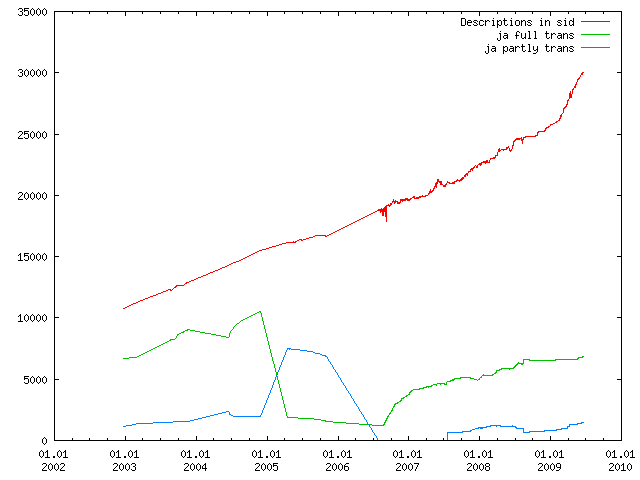
\includegraphics[width=1\hsize]{image200906/stat-trans-sid-ja.png}
 
\end{frame}

\begin{frame}{DDTSS の Greasemonkey を作成した}
 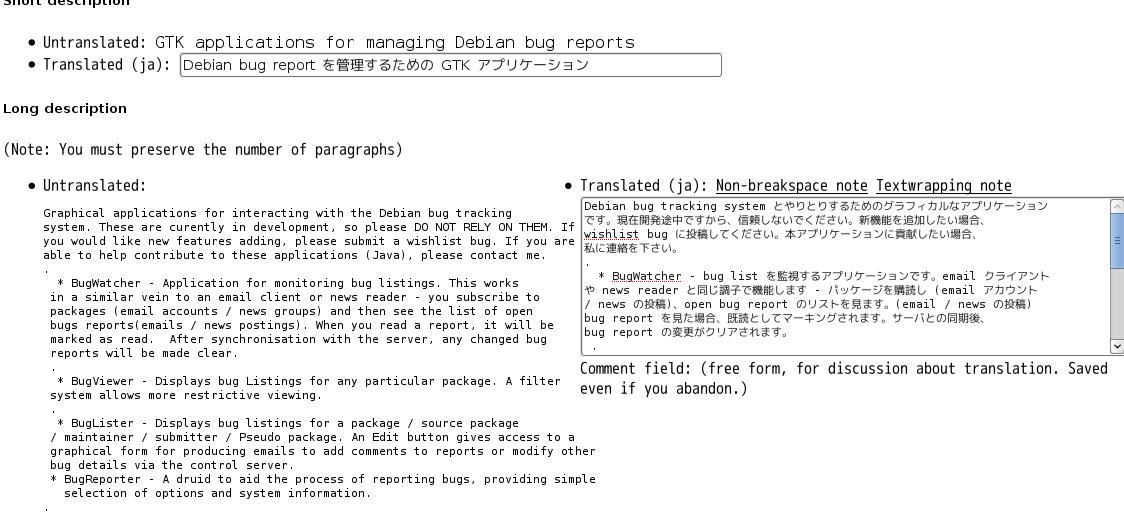
\includegraphics[width=1.2\hsize]{image200906/ddtss-greasemonkey.png}
\end{frame}

\begin{frame}[containsverbatim]{Firefox Greasemonkey}
\begin{commandline}
 apt-get install iceweasel-greasemonkey
\end{commandline}
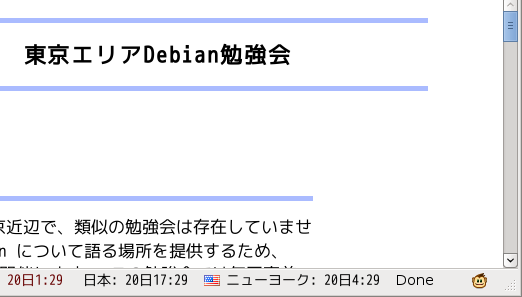
\includegraphics[width=6cm]{image200906/greasemonkey.png}
\end{frame}

\begin{frame}[containsverbatim]{greasemonkey script content}

\begin{commandline}
// ==UserScript==
// @name           DDTP two-panes
// @namespace      ddtptwo
// @description    Display DDTP in two-panes mode
// @include        http://ddtp.debian.net/ddtss/index.cgi/*/translate/*
// @include        http://ddtp.debian.net/ddtss/index.cgi/*/forreview/*
// ==/UserScript==

(function() {
    // Get the third UL, and name it floatie.
    document.getElementsByTagName("ul")[2].setAttribute("id", "floatie");
    // Do not show the diff since it's rather useless.
    var style =
	<><![CDATA[
		   div.diff {
		       display: none;
		   }
		   ul#floatie > li {
		       float: left;
		       width: 50%;
		   }
		   ul#floatie * pre {
		       font-size: 70%;
		   }
		   ul#floatie * textarea {
		       font-size: 70%;
		   }
		   ]]></>
    GM_addStyle(style);
})()
\end{commandline}

\end{frame}

\begin{frame}{事前課題}

DDTSS (先月のPDF資料 今月のPDF資料参照)でいくつか(2個以上)Debianパッケージの説明文を翻訳してみて、いくつか(2個以上)レビューしてみて、そこでの

\begin{enumerate}
 \item 作業に適用した主要な方法
 \item 発見した課題
 \item 方法の改善案の提案をしてください。
\end{enumerate}

\end{frame}

{\footnotesize
%; whizzy-master ../debianmeetingresume200906.tex
% $B0J>e$N@_Dj$r$7$F$$$k$?$a!"$3$N%U%!%$%k$G(B M-x whizzytex $B$9$k$H!"(Bwhizzytex$B$,MxMQ$G$-$^$9!#(B

\begin{prework}{$B>e@n=c0l(B}
...
\end{prework}



\begin{prework}{$B@nK\7rB@O:(B}
\preworksection{$BE,MQ$7$?<gMW$JJ}K!(B}

2009/06$B$N;qNA$N!V(BDDTSS$B$NK]Lu:n6H$N>R2p!W$r;29M$K!"(B
DDTSS $B$K%f!<%6!<EPO?$7!"?7$7$$K]Lu!&=$@5!&%l%S%e!<$r(B3$B$D$:$D9T$$$^$7$?!#(B


\preworksection{$BH/8+$7$?2]Bj(B}

\begin{itemize}
 \item "Accept with changes" $B$9$k$H!"%l%S%e!<%W%m%;%9$,$d$jD>$7$K$J$k$N$G!"$A$g$C$H$7$?=$@5(B ($B6gFIE@$NDI2C$J$I(B) $B$,$G$-$J$$(B
 \item ($B$=$NA0$N9F$H$N:9J,$@$1$G$O$J$/(B) $B:G?79F$b8+$?$$(B
 \item $BK]Lu$N4p=`$,$o$+$i$J$$$N$G!"(BSubmit$B$7$FNI$$$N$+<+?.$,;}$F$J$$(B
 \item DDTSS$B$N%5!<%P>ZL@=q$,IT@5(B
 \item Alias$B$N%k!<%k$,EPO?;~$H%m%0%$%s;~$H$G0[$J$k(B ($BEPO?;~$O(B "at least 4 letter long" $B$G%m%0%$%s;~$O(B "at least 6 letter long")
\end{itemize}

3 $BE@L\$O?4M}E*$JLdBj$G$9$,!"(B
$B$I$N%l%Y%k$NK]Lu$r5a$a$i$l$F$$$k$N$+$o$+$i$J$$$N$G!"(B
Submit $B$r$?$a$i$C$F$7$^$$$^$7$?!#(B
($B$H$O$$$(!":G=*E*$K$O(B Submit $B$7$^$7$?$,!#(B)
$B8mLu$,$J$$$N$OEvA3$H$7$F$b!"@lLgMQ8l$NLu$d!"(B
$BF|K\8l$H$7$F$N<+A3$5$J$I!"K]Lu$N<A$,5$$K$J$C$F$7$^$$$^$9!#(B

\preworksection{$BDs0F$9$kM}A[A|(B($B%D!<%k$H$+(B)$B!"6&M-$7$?$$>pJs(B}

$B>e5-2]Bj$N(B 1 $BE@L\$NBP:v$H$7$F!"(B
"Change and restart review process" $B$H(B "Accept with minor changes" $B$H$N(B
2 $B$D$,J,$+$l$F$$$l$PNI$$$H;W$$$^$9!#(B
$B!V$o$:$+$J=$@5$G$b!"%l%S%e!<%W%m%;%9$r$d$jD>$9!W$H$$$&$N$O!"(B
$B87L)@-$rJ]$D$?$a$K$OI,MW$G$9$,!"(B
"The number of translations pending review has gotten quite large." $B$H$$$&>u67$G!"(B
$B6gFIE@0l$DD>$9$?$S$K!"$^$?(B 3 $B?M$N%l%S%e!<%o$,I,MW$K$J$k$N$O8=<BE*$G$O$J$$$H;W$$$^$9!#(B
$B5U$K!"%l%S%e!<%o$,$A$g$C$H$7$?=$@5$r$"$-$i$a$k$3$H$G!"(B
$B%I%-%e%a%s%H$,$A$g$C$HFI$_$K$/$/$J$k$N$O;DG0$G$9!#(B


\end{prework}

\begin{prework}{$B$^$($@$3$&$X$$(B}

\preworksection{$BE,MQ$7$?<gMW$JJ}K!(B}

$B$3$3$G$N(B''$BJ}K!(B''$B$,2?$r0U?^$7$F$$$k$N$+$,J,$+$i$J$$$N$G!"%D!<%k$N;H$$J}$G(B
 $B$O$J$/!"K]Lu$N$d$jJ}$H$$$&4QE@$G=q$-$^$9!#K]Lu$N$d$jJ}<+BN$O!"K]LuDL?.(B $BJL:}!X?N(B
 $BJ?OBIW>.O@=8(B $BK]Lu$N%3%D!Y(B
 \footnote{\url{http://homepage3.nifty.com/hon-yaku/tsushin/bn/200209SAp2.pdf}}
 $B$r;29M$K$7$^$7$?!#%3%D$O?'!9$"$k$h$&$G$9$,!"$$$/$D$b0U<1$9$k$N$OFq$7$$(B
 $B$N$G!"<!$N;0E@$@$1$O0U<1$9$k$h$&$K$7$^$7$?!#(B

\begin{itemize}
 \item $BD>Lu$K$O$7$J$$$G!"F|K\8l$H$7$F$o$+$j$d$9$$J8>O$r?4$,$1$k!#(B
 \item $BD9J8$GJ,$+$j$E$i$1$l$P!"C;J8$KJ,3d$7$F$_$k!#(B
 \item $B7AMF;l$,O"H/$5$l$F$$$kItJ,$O0U?^E*$KLu$5$J$$!#(B
\end{itemize}

\preworksection{$BH/8+$7$?2]Bj(B}

 $B$^$:!"%7%9%F%`E*$J$3$H!#(B

 $B%m%0%$%s$7$J$/$F$b(B $B%l%S%e!<!"=$@5$G$-$F$7$^$C$?$N$G!"(BID $B$r:n$C$F$$$?$K(B
 $B$b4X$o$i$:!"(Bcokkie $B$K;D$C$?>pJs$G%"%/%;%9$7$F$$$k$N$+$H;W$$$=$N$^$^(B
 Accept $B$9$k$H!"(BID $B$,(B IP $B%"%I%l%9$K$J$C$F$7$^$&$H$$$&$A$g$C$H%^%L%1$J<+(B
 $BBN$K!#(B


 $B$b$&0l$D$O!"@lLgMQ8l$K$D$$$F!#85!9Bg3X$,@8J*3X2J$G$7$?$N$G!"@8J*4XO"$N(B
 $B@lLgMQ8l$K8BDj$7$FOC$r$7$^$9!#3X@8;~J,$K!"0lHV:$$C$?$N$O1Q8l$NJ8=q$7$+(B
 $B$J$$$3$H$G$O$J$/$F!"JQ$JK]Lu$N$5$l$+$?$r$7$F$$$kMQ8l!"FC$K%+%?%+%J$KK](B
 $BLu$5$l$F$$$kMQ8l$G$9!#(B

 $B@lLgMQ8l$rD4$Y$k$N$K$O!"DL>o!"@lLgMQ8l$N<-=q$r;H$$$^$9!#@8J*$@$H@8J*3X(B
 $BA4HL!"@82=3X!"7OE}J,N`3X!"J,;R@8J*3X!"$J$I$J$I!"3FJ,Ln$G@lLg$N<-=q$,$"(B
 $B$j$^$9$,!"JQ$KK]Lu$5$l$F$$$k$H!":w0z$+$i0z$/$3$H$,$G$-$^$;$s!#$G$9$N$G!"(B
 $B@lLgMQ8l$rD4$Y$k$H$-$O!"86J8!J1Q8l$+!"3XL>$G;H$o$l$k%i%F%s8l!K$GD4$Y$k(B
 $B$N$,4pK\$G$9!#(B

\preworksection{$BDs0F$9$kM}A[A|(B($B%D!<%k$H$+(B)$B!"6&M-$7$?$$>pJs(B}

 $BA0<T$K$D$$$F$O!"(BDDTSS$B$K%m%0%$%s$7$J$$$HJQ99$G$-$J$$$h$&$K%j%/%(%9%H$r=P(B
 $B$9$N$,$h$$$N$G$7$g$&$+!D!#(B


 $B8e<T$K$D$$$F$O!"$"$1$I$5$s$,:#2s$*OC!"Ds8@$7$F$/$@$5$k$H;W$$$^$9$,!"0lHL(B
 $B?M8~$1$KK]Lu$O$9$k$b$N$N!"86J8$O3g8L=q$-$J$I$G8e$m$K;D$7$F$*$/$N$,<B:](B
 $B$K;H$&%f!<%6!J$=$NJ,Ln$N@lLg2H!K$K$O?F@Z$@$H;W$$$^$9!#(B

\end{prework}


\begin{prework}{$B$"$i$-$d$9$R$m(B}

\preworksection{$BE,MQ$7$?<gMW$JJ}K!(B}

$B$H$/$K$J$$$+$J$"!#$R$?$9$iK]Lu!#(B

\preworksection{$BH/8+$7$?2]Bj(B}

$B%Q%C%1!<%8L>$$$-$J$j$8$c$J$/$F!"%Q%C%1!<%8$N=jB0$9$k(Bsection$B$,$+$+$l$F$$$k$H3Z$J(B
$B$N$K$J$"!"$H;W$$$^$7$?!#(B
review$B$,$*$b$$$N$[$+4JC1$H$$$&$+!"$Y$D$K(Bdd$B$,$R$H$j$b4X78$7$J$/$F$b$$$$$s$G$9$M!#(B
$B$"$k0UL#$*$I$m$-$+$b!#(B

\preworksection{$BDs0F$9$kM}A[A|(B($B%D!<%k$H$+(B)$B!"6&M-$7$?$$>pJs(B}

$BD6$`$+$7(B(1997$B$3$m(B)$B$K$3$N<j$N:n6H$r$7$?$H$-$H$O$<$s$<$s0c$$$^$9$M!#(B
$B$G$b!"$"$$$F$k;~4V$K$d$j$?$$$H$-$b$"$k$N$G%*%s%i%$%s$G$O$J$/%P%C%A=hM}$G$-$k;EAH(B
$B$b$N$3$C$F$k$H$&$l$7$$$+$J$H!#(B

\end{prework}


}

\emtext{bsdstats を Debianize した}

\emtext{kFreeBSD}

\begin{frame}{次回勉強会のテーマ}
\begin{itemize}
 \item 会場はスペイン
 \item その次は?
\end{itemize}
\end{frame}

\begin{frame}{宴会場所}
\begin{itemize}
 \item 宴会場所\\
       本日の宴会場所は「安安」です。\\
       21:00 開始です。
 \item 片付け\\
       部屋を片付けるのにご協力ください。
\end{itemize}
\end{frame}

\end{document}

;;; Local Variables: ***
;;; outline-regexp: "\\([ 	]*\\\\\\(documentstyle\\|documentclass\\|emtext\\|section\\|begin{frame}\\)\\*?[ 	]*[[{]\\|[]+\\)" ***
;;; End: ***
